%%% LaTeX Template: Article/Thesis/etc. with colored headings and special fonts
%%%
%%% Source: http://www.howtotex.com/
%%% Feel free to distribute this template, but please keep to referal to http://www.howtotex.com/ here.
%%% February 2011
%%%
%%% Last updated September 2018 by CDM

%%%  Preamble
\documentclass[11pt,letterpaper]{article}
\usepackage[margin=1.0in]{geometry}
\usepackage[T1]{fontenc}
\usepackage[bitstream-charter]{mathdesign}
\usepackage[latin1]{inputenc}					
\usepackage{amsmath}						
\usepackage{xcolor}
\usepackage{cite}
\usepackage{hyphenat}
\usepackage{graphicx}
\usepackage{float}
\usepackage{subfigure}
\usepackage{sectsty}
\usepackage[compact]{titlesec} 
\usepackage[tablegrid]{vhistory}
\usepackage{url}


\allsectionsfont{\color{accentcolor}\scshape\selectfont}

%%% Definitions
\definecolor{accentcolor}{rgb}{0.0,0.0,0.5} 
\newcommand{\teamname}{The Brew Crew}
\newcommand{\productname}{Beverage Management}
\newcommand{\coursename}{CSE 4316: Senior Design I}
\newcommand{\semester}{Summer 2020}
\newcommand{\docname}{Project Charter}
\newcommand{\department}{Department of Computer Science \& Engineering}
\newcommand{\university}{The University of Texas at Arlington}
\newcommand{\authors}{Kunal Samant \\ Nirjal Phaiju \\ Sima Raymajhi \\ Bishal Paudel \\ Lokendra Chettri}

%%% Headers and footers
\usepackage{fancyhdr}
	\pagestyle{fancy}						% Enabling the custom headers/footers
\usepackage{lastpage}	
	% Header (empty)
	\lhead{}
	\chead{}
	\rhead{}
	% Footer
	\lfoot{\footnotesize \teamname \ - \semester}
	\cfoot{}
	\rfoot{\footnotesize page \thepage\ of \pageref{LastPage}}	% "Page 1 of 2"
	\renewcommand{\headrulewidth}{0.0pt}
	\renewcommand{\footrulewidth}{0.4pt}

%%% Change the abstract environment
\usepackage[runin]{abstract}			% runin option for a run-in title
%\setlength\absleftindent{30pt}			% left margin
%\setlength\absrightindent{30pt}		% right margin
\abslabeldelim{\quad}	
\setlength{\abstitleskip}{-10pt}
\renewcommand{\abstractname}{}
\renewcommand{\abstracttextfont}{\color{accentcolor} \small \slshape}	% slanted text

%%% Start of the document
\begin{document}

%%% Cover sheet
{\centering \huge \color{accentcolor} \sc \textbf{\department \\ \university} \par}
\vspace{1 in}
{\centering \huge \color{accentcolor} \sc \textbf{\docname \\ \coursename \\ \semester} \par}
\vspace{0.5 in}
\begin{figure}[h!]
	\centering
   	
\includegraphics[width=0.40\textwidth]{images/beverage}
\end{figure}
\vspace{0.5 in}
{\centering \huge \color{accentcolor} \sc \textbf{\teamname \\ \productname} \par}
\vspace{0.5 in}
{\centering \large \sc \textbf{\authors} \par}
\newpage


%\vspace{1 in}
%\centerline{January 13th, 2012}
%\newpage

%%% Revision History
\begin{versionhistory}
	  \vhEntry{0.1}{07.08.2020}{KS}{document creation}
	  \vhEntry{0.2}{07.09.2020}{SR, NP, BP, LC}{sections added (4,7,8,9,10,13 left)}
	  \vhEntry{0.3}{07.10.2020}{NP, LC}{sections added (4,13 left)}
	  \vhEntry{0.4}{07.11.2020}{SR, BP, NP, LC, KS}{sections 4 and 13 added}
\end{versionhistory}
\newpage

%%% Table of contents
\tableofcontents
\newpage

%%% List of figures and tables (optional)
\listoffigures
%\listoftables
\newpage
\setcounter{table}{0}

%%% Agile project charter sections
\section{Vision}
The vision defines the "Why" of the project. This is the higher purpose, or the reason for the project's existence. This section should avoid mentioning implementation details, and focus more on what the current problem is and what would be gained if the problem were to be solved. In short, the is the reason that you are going to be working on something, not the method(s) that you will be employing.
\section{Mission}
Our team aims to develop a well-managed and easy to navigate application for managing
alcoholic beverage. Apart from easy navigation, we aim to develop a systematic way of keeping
tabs of the inventory with maximum accuracy. Through our application, users will be able to
successfully track and categorize the alcohol products they have. Our application provides a
chance for the users track the financial losses that may have occurred by accidental damage or
theft of a product. Our product aims to attract individuals who love collecting variety of alcohol
product, alcohol beverage companies and businesses that sell alcohol.
\\
\\
The tools that we will be using while implementing the project are:
\begin{itemize}
  \item android studio
  \item iOS
  \item API calls
\end{itemize}
\section{Success Criteria}
The app will be used to manage a vast quantity of beverage items. The main priority of the app will be to 
properly manage the inventory which is scanned by the user. Additionally, for the first delivery, 
the app should support android and iOS based applications which will have access to the camera. 
Further features, such as, notifications, sounds, animations, and data will be added after the initial delivery.
The final app should be able to store the read, interpret and store the beverage information in shelves (which will be added by the user) 
and send notifications to the user about expiry dates amongst other information.
\\
\\
After the beverage is scanned:
\begin{itemize}
  \item notifications will be issued
  \item space limit will be monitored
\end{itemize}

\newpage

%%% Remaining project charter sections
\section{Background}
We all have unique hobbies and habits. Some people enjoy doing outdoor activities whereas other enjoy doing indoor activities such as collecting things that they like. Different people have different kinds of interests such as collecting antique coins, seashells, alcoholic beverages, etc. We are focused and dedicated to work on a project that helps those have an interest in collecting various beverages by allowing them to organize their beverage properly. That is why we have decided to work on the app called The Beverage Management which was inspired by Dr. Conly's idea. This app will help an individual as well as small businesses to keep track of the beverages in timely manner. This app will allow a customer to keep the track of name, expiry date, and location of the beverage which will make it easier for them to find the specific one that they are looking for. This app will save people's time and money as it will keep the beverages information date updated and will allow them to consume the beverage before the expiry date.
\section{Related Work}
Discuss the state-of-the-art with respect to your product. What solutions currently exist, and in what form (academic research, enthusiast prototype, commercially available, etc.)? Include references and citations as necessary using the \textit{cite} command, like this \cite{Rubin2012}. If there are existing solutions, why won't they work for your customer (too expensive, not fast enough, not reliable enough, etc.). This section should occupy 1/2 - 1 full page, and should include at least 5 references to related work. All references should be added to the \textit{.bib} file, fully documented in IEEE format, and should appear in the \textit{references} section at the end of this document (the IEEE citation style will automatically be applied if your reference is properly added to the \textit{.bib} file).

ProTip: Consider using a citation manager such as Mendeley, Zotero, or EndNote to generate your \textit{.bib} file and maintain documentation references throughout the life cycle of the project.
\section{System Overview}
Lots of beverage consumers lose track of their collection sof drinks and this can lead to a major loss of money and shelf space. We 
decided to use a dataset which contains the data for a variety of rare beer to design our drinks database. The user will 
be able to scan the beer the purchased using an in-built barcode scanner in the app and assign the drink to an empty 
portion of the shelf.  

    Our system will need access to the phones camera, which will only be active when the user wants to scan the bar code.
The system will search for the information of the drink using the barcode in the dataset and populate the shelves on the application with the required data.

    The expiration date of the beer and the number of that type of beer in the shelves will be kept track of so as to handle the user requests, and also 
send push notifications to the user when the beer is low on supply or about to expire.

    Furthermore, the user can modify the functionality of the app (i.e the notifications sound, details of each shelf) within the app.

\begin{figure}[ht]
    \centering
    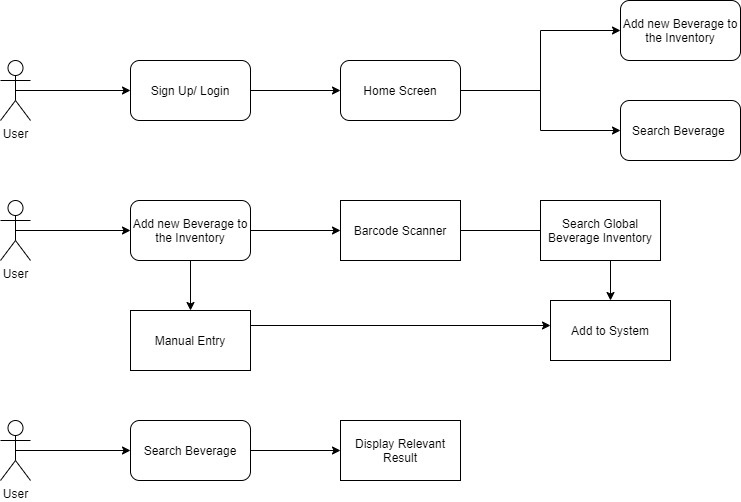
\includegraphics[width=0.5\textwidth]{images/systemoverview}
    \caption{High Level system overview of major system components}
\end{figure}
\section{Roles \& Responsibilities}
Stakeholders of our project would be Dr. Christopher Conly and CSE department, Points of contact from the sponsor or customer side and Scrum Master is Dr. Christopher Conly.
\\
The team members are Bishal Paudel, Kunal Samant, Nirjal Phaiju, Sima Ryamajhi, and Lokendra B. Chhetri. As Miyamoto Musashi said, "Fixation is the way to death. Fluidity is the way to life." So, to give life to this project, we decided to gyrate our Scrum Master and team leader in every phase. Initially, we decided to appoint Kunal as a team lead and Scrum Master as Dr. Conly.
\\
For this phase, Kunal and Nirjal will be working on Backend whereas Bishal and Lokendra will work on GUIs and frontend. Sima will work as a risk management lead. As a team, we will be giving 100{\%} on the tasks we are assigned and also helping each other out.

\section{Cost Proposal}
This section contains the approximate budget for the project, where that money will come from, and any other support. This text should be replaced with a discussion and justification of major expenses, but not the actual monetary amounts (that will go in the preliminary budget section below). 

\subsection{Preliminary Budget}
Include a high level budget table for components, fabrication, software licensees, development hardware, etc. This should be in a tabular format broken up into appropriate line items. 

\subsection{Current \& Pending Support}
What are all of the funding sources for the project, and are there any potential funding sources that haven't been secured yet? List all funding sources (including the default funding amount provided by the CSE department) and their dollar amounts.
\section{Facilities \& Equipment}
What lab space, testing grounds, makerspaces, etc. will you need to complete the project? Will you require any specific equipment, and if so, where will you get it (borrow, lease, purchase, outsource, already present in the lab, etc.). This section should occupy 1/2 page.
\section{Assumptions}
The following list contains critical assumptions related to the implementation and testing of the project:

\begin{itemize}
  \item The budget provided by the CSE department will be enough to deliver and smooth and working application.
  \item The members of the team are familiar with front-end and back-end aspect of software development which 
  will be critical for balanced distribution of the workload among group members.
  \item No external hardware will be needed in order to complete our project
  \item Users of the application will have access to internet and camera.
  \item The application will focus on android users.
  \item A suitable and affordable API will be found in order to successfully implement barcode scanner.
\end{itemize}
\section{Constraints}
The following list contains key constraints related to the implementation and testing of the project. 

\begin{itemize}
  \item A team of five members will work on the project.
  \item All the team meetings will be done through Microsoft Teams software.
  \item The development costs must be less than \$800. 
  \item Final prototype demonstration must be completed by August 12, 2020. 
  \item Access to online beverage inventory database will be made available during the development phase of the application.
  \item Application will be made using android OS.

\end{itemize}

\section{Risks}
This section should contain a list of at least 5 of the most critical risks related to your project. Additionally, the probability of occurrence, size of loss, and risk exposure should be listed. For size of loss, express units as the number of days by which the project schedule would be delayed. For risk exposure, multiply the size of loss by the probability of occurrence to obtain the exposure in days. For example:

The following high-level risk census contains identified project risks with the highest exposure. Mitigation strategies will be discussed in future planning sessions.

\begin{table}[h]
\resizebox{\textwidth}{!}{
\begin{tabular}{|l|l|l|l|}
\hline
 \textbf{Risk description} & \textbf{Probability} & \textbf{Loss (days)} & \textbf{Exposure (days)} \\ \hline
 Availability of X sensor module due to contractor delay  & 0.50 & 20 & 10 \\ \hline
 Outdoor testing grounds are not available  & 0.20 & 14 & 2.8 \\ \hline
 Internet access not available at installation site  & 0.30 & 9 & 2.7 \\ \hline
 Delays in shipping from overseas vendors  & 0.10 & 20 & 2.0 \\ \hline
 Certification delays at compliance testing facility & 0.15 & 10 & 1.5 \\ \hline
\end{tabular}}
\caption{Overview of highest exposure project risks} 
\end{table}
\section{Documentation \& Reporting}
%%% In this section, you will describe all of the various artifacts that you will generate and maintain during the project life cycle. Describe the purpose of each item below, how the content will be generated, where it will be stored, how often it will be updated, etc. Replace the default text for each section with your own description. Reword this paragraph as appropriate.

\subsection{Major Documentation Deliverables}
We will divide the work between all the team members, and complete our individual part. Each team member will be responsible for maintaining their own part and updating if necessary. The final document will be reviewed by the team before submitting.  
\subsubsection{Project Charter}
The initial version of the charter will be revised by the group before submitting it on July 12th, 2020. The charter will be updated as per the changes made in this project. Also, feedback from the team member and Professor will be taken into consideration, and the charter will be updated before the final version. The final version will be delivered on December 1st, 2020.
\subsubsection{System Requirements Specification}
We will write all the requirements for the project and make sure with our customer/Professor to check that if all the requirements have been included before starting on project. When changes are made in the projects, requirements will be updated and maintained. While making the projects we will contact customer to make sure that our software meets customer all needs. We will make required changes in the requirements from the feedback of the customer. The final version will be submitted on July 27th, 2020.
\subsubsection{Architectural Design Specification}
The initial document will be submitted on-----Before starting any of the development in the project, we will make the architectural design layout and submit it to the customer. After the feedback of the customer on its we will start to work on development. There might be few changes in this document after the feedback of the customer and Professor.  This document will be updated when there are any changes made in the design. The final version will be delivered on August 20th, 2020.
\subsubsection{Detailed Design Specification}
Detailed design specification will be started after we have requirements specification and architectural design specification so that we will have everything to start working on. The layout for the detailed design will be shown to the customer and Professor for the validation. The initial version will be submitted on September 21st, 2020. There will be changes made in this document over the time. This document will be updated when there are some changes made in the design of the project after the validation with the customer. The final version will be submitted on December 1st, 2020.




\subsection{Recurring Sprint Items}
\subsubsection{Product Backlog}
We will add items to the product backlog based on their level of importance and dependencies. We will
decide what elements are a must-have to be completed first while also making sure items that are a
critical part of the other parts of the software are placed at a higher priority. We will decide as a group
what needs to get done and in what order. At the moment, we haven't narrowed down exactly what
software we will use to maintain the backlog.
\subsubsection{Sprint Planning}
Each sprint will be decided based off of the previous sprint and what is needed to be done. There will be roughly 4 sprints.

\subsubsection{Sprint Goal}
Our sprint goal will be decided by our group.
\subsubsection{Sprint Backlog}
The sprint backlog will be similar to the product backlog and the sprints will be decided based on the remaining tasks,
ordered based on their priority.
\subsubsection{Task Breakdown}
Each task will be discussed and then assigned to a specific member in order to ensure a fair distribution and based on the members
strengths and weaknesses.
\subsubsection{Sprint Burn Down Charts}
The team lead for that specific sprint will be tasked to generate a Burn Down chart:

\begin{figure}[h!]
    \centering
    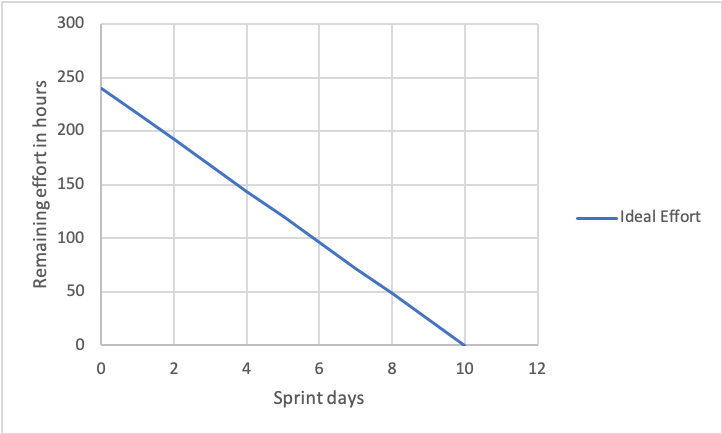
\includegraphics[width=0.6\textwidth]{images/burndown}
    \caption{Example sprint burn down chart}
\end{figure}

\subsubsection{Sprint Retrospective}
At the end of each sprint we will gather together and meet to discuss what will be needed in further sprints. The sprints wont have specific due dates
as the team would be able to communicates the status of their tasks.
\subsubsection{Individual Status Reports}
We will report to each other and communicate regularly about the updates on the project. We will note important points which will need to be discussed prior to deadlines.
\subsubsection{Engineering Notebooks}
The engineering notebook should be updated whenever ideas related to the project arise. Hopefully,
there would be a few updates between each meeting that we have regarding large changes to the project.


\subsection{Closeout Materials}
The following materials, in addition to major documentation deliverables, will be provided to the customer upon project closeout. Remove this paragraph from your draft, but leave the heading.

\subsubsection{System Prototype}
The Final System Prototype will have an android application that is well tested and properly functional. 
The Prototype shall be demonstrated to relevant stakeholders before the end of Senior Design 2. The team will 
be meeting with the project supervisor and customer on several occasions for Prototype Acceptance Test. This 
will help our team to ensure that we are moving in the right direction. There will be no demonstrations off-site 
therefore, no need for Field Acceptance Test.
\subsubsection{Project Poster}
The poster of our project will include our applications vision, mission and guidelines for installing 
the application. The Dimension of the poster approximately 20-30 inches wide and 30-40 inches tall. The poster 
will be delivered one day before the final presentation day of Senior Design 2.
\subsubsection{Web Page}
Web Page will contain the basic information of your project. This web page will help the readers learn more about 
the application and the team behind the application. The web page will consist of the team's vision, mission, 
background and introduction to the team members.
\subsubsection{Demo Video}
The Demo video will show the viewers how to install and use the software. 
It will inform the users about the major features of the application. The video will be 3-6 minutes long.
\subsubsection{Source Code}
The source code will be pushed to github repository periodically. The source code will only be available 
for team members until the project is complete. After the completion of project, the source code will be 
available to the sponsors of the project, and decision of making code available to public will be decided later.
\subsubsection{Source Code Documentation}
We will present our documentation in html format, with documentation for each function or parts of
the code.
\subsubsection{Installation Scripts}
The app will be available in app store so it will be very use to download and install.
\subsubsection{User Manual}
This app will be user friendly and very easy to use. The app will have short introduction video explaining 
about its features and how this app works so it will easy for everyone to use this app.
\newpage

%%% References
\linespread{1.3}\selectfont
\bibliographystyle{IEEEtran}
\section{References}
\bibliography{reference/refs}{}

\end{document}